% This document is part of the transientdict project.
% Copyright 2013 the authors.

\documentclass[12pt]{emulateapj}
\usepackage{graphicx}
\usepackage{subfigure}
%\usepackage{epsfig}
\usepackage{times}
\usepackage{natbib}
\usepackage{amsfonts}
\usepackage{amsmath}
\usepackage{amsbsy}
%\usepackage{hyperref}
%\usepackage[stable]{footmisc}
%\usepackage{color}
%\bibliographystyle{apj}

\newcommand{\project}[1]{\textsl{#1}}
\newcommand{\Fermi}{\project{Fermi}}
\newcommand{\RXTE}{\project{RXTE}}
\newcommand{\given}{\,|\,}
\newcommand{\dd}{\mathrm{d}}
\newcommand{\counts}{y}
\newcommand{\pars}{\theta}
\newcommand{\mean}{\lambda}
\newcommand{\likelihood}{{\mathcal L}}
\newcommand{\Poisson}{{\mathcal P}}
\newcommand{\Uniform}{{\mathcal U}}
\newcommand{\bg}{\mathrm{bg}}
\newcommand{\word}{\phi}

\begin{document}

\title{Dissecting Magnetar Variability with Bayesian Hierarchical Models}

\author{D. Huppenkothen\altaffilmark{1, 2}, B. Brewer\altaffilmark{}, D. Hogg\altaffilmark{}, I. Murray\altaffilmark{}, M. Frean\altaffilmark{}, A. L. Watts\altaffilmark{1}, Y.Levin\altaffilmark{},  L. Heil\altaffilmark{1}, C. Kouveliotou\altaffilmark{3,4}}

 
\altaffiltext{1}{Anton Pannekoek Institute for Astronomy, University of
  Amsterdam, Postbus 94249, 1090 GE Amsterdam, the Netherlands}
  \altaffiltext{2}{Email: D.Huppenkothen@uva.nl}
\altaffiltext{3}{Astrophysics Office, ZP 12, NASA-Marshall Space Flight Center, Huntsville, AL 35812, USA}
\altaffiltext{4}{NSSTC, 320 Sparkman Drive, Huntsville, AL 35805, USA}

\altaffiltext{}{Monash Center for Astrophysics and School of Physics, Monash University, Clayton, Victoria 3800, Australia}

%\section*{A model for magnetar bursts}

%\noindent
%Huppenkothen, Murray, Hogg, Brewer, Frean \\
%\textsl{2013 December}

\begin{abstract}
Magnetars are whatever and people need whatever.
Magnetars produce bursts,
  each of which appears to be composed of a set of one or more spikes.
Here we build a probabilistic generative model for the \Fermi\ GBM photon data on Magnetar bursts.
The spikes appear to be somewhat asymmetric
  (rise looks different from decay),
  have various amplitudes,
  but have widths that appear to be similar \emph{within} each burst.
We model each burst as being composed of a mixture of spikes,
  where each spike is a scaled, stretched, and shifted version of a universal dimensionless function.
We perform probabilistic inference with a Poisson likelihood and vague priors to determine
  the positions, amplitudes, and positions of the spikes,
  the width of the spikes in each burst,
  and the shape of the dimensionless spike function.
The phenomenology of spike multiplicity, shape, and width is discussed.
\end{abstract}

\keywords{pulsars: individual (SGR J1550-5418), stars: magnetic fields, stars: neutron, X-rays: bursts, methods:statistics}

\section{Introduction}

With current and upcoming telescopes monitoring the sky regularly across the entire electromagnetic spectrum, time domain astronomy is emerging as one of the key fields in which major new discoveries are being made.  A large fraction of astrophysical sources are known to be variable. The timescales span more than five orders of magnitude: fast oscillations in X-ray binaries (XRBs) change over milliseconds \citep[e.g.][]{xrb_khzqpos}, while red giants are believed to change over decades or even centuries \citep[e.g.][]{dasch_giants}. Variability studies have the potential to unravel fundamental physical processes: studying variability in XRBs can help us unravel accretion processes and constrain theories of viscosity. Similarly, giant flares from magnetars have the potential to map the neutron star interior via neutron star seismology. 

While much of the variability exhibited for example in XRBs is accessible by standard Fourier methodology, this is not true for an important group of sources: for any transients with complex temporal structure where the relevant time scales of interest are of the same order as the typical time scales in the system,  this variability introduces considerable systematic errors into inferences made from this type of data with standard methods. Three examples stand out particularly: solar flares, $\gamma$-ray bursts (GRBs) and magnetar bursts. All three phenomena are characterised by emission at high (X-ray to soft $\gamma$-ray$) energies, bursts lasting from $\sim 1/10$ of a second to hundreds of seconds, and a complex temporal structure that varies strongly from burst to burst (for an example, see \ref{fig:burst example}). Fourier methods are hampered by the lack of knowledge of the overall structure of the burst, and consequently the lack of knowledge of both the shape and the statistical distribution of powers in the periodogram at low frequencies. Conversely, it is difficult to postulate a common model applicable to a large sample of light curves of these sources. Any light curve model must be flexible enough to account for differences between bursts. At the same time, there is little understanding of the underlying physical processes leading to variability in these bursts to inform a choice of model. Here, we aim to develop a probabilistic model for highly variable transient events, based on a decomposition of the light curve into simple shapes, without knowing the number of components in the model a priori. We demonstrate the power of this approach on a large sample of magnetar bursts, and, for the first time, connect variability in magnetar bursts to the time scales thought to govern the underlying physics.


Neutron stars, the ultra-dense compact remnants of core-collapse supernovae, are the prime laboratory for studying nuclear 
physical processes in a parameter regime of density and pressure inaccessible to experiments on Earth. 
Among the veritable zoo of neutron star phenomena, two stand out for their peculiar parameters: Soft Gamma Repeaters (SGRs),
named after their hallmark recurring bursts in hard X-rays, and Anomalous X-ray Pulsars (AXPs), persistent pulsating X-ray
sources with a conspicuous paucity of radio counterparts (although a total of three sources from both groups now
have confirmed radio detections). 

While SGRs and AXPs were detected as separate phenomena, they share common properties: slow spin periods between
$2 - 12 \, \mathrm{s}$, coupled with generally high period derivatives, lead to large inferred dipole magnetic fields of
the order of $10^{14} \, \mathrm{G}$, well above the quantum-critical limit $B_{\mathrm{QED}} = 4.4 \times 10^{13} \, \mathrm{G}$,
where quantum effects such as pair production and photon splitting become important (although three sources have been 
identified with properties similar to SGRs and AXPs, but inferred dipole fields below this limit). 

Both AXPs and SGRs are believed to be the observable phenomena of the same underlying physical system: a highly magnetised
neutron star, also called a magnetar. In the standard scenario, the observable X-ray emission, both persistent emission and bursts, 
is powered by the slow evolution and decay of the source's strong magnetic field, instead of the loss of rotational energy as 
is generally the case for standard radio pulsars. 

SGR bursts are of particular interest for a variety of reasons. Most importantly, the observation of three giant flares, catastrophic
outbursts in hard X-rays of energies up to $10^{47} \, \mathrm{erg}$, and the associated detection of quasi-periodic oscillations (QPOs)
in the tails of these flares, have opened up a potential new way to look into the neutron star interior via asteroseismology. In the standard 
model, these giant flares are caused by a catastrophic re-ordering of the neutron star's internal field. As the magnetic field lines, frozen into
the solid crust, move, the crust responds by fracturing when its breaking strain is exceeded by the forces exerted by the magnetic field.
The energy released in this process is both released into the magnetosphere, where it forms a pair plasma that slowly radiates away and
produces the observed emission, as well as seismic waves throughout the star. The frequencies of the oscillatory modes depend on
the nuclear physics of the star's crust and core, making them a prime diagnostic for the conditions inside the star.

While giant flares are relatively rare phenomena (we have only observed $3$ in the last $35$ years), magnetars also show a complex
behaviour of emitting much smaller, shorter recurrent bursts. These bursts are of the order of $<1\mathrm{s}$ long, with energies
generally between $10^{38}\,\mathrm{erg}$ and $10^{41}\,\mathrm{erg}$, and have a complex temporal structure with single or
multiple peaks that differs from one burst to the next. They are observed either appearing individually, or in burst 
storms, where tens or hundreds of bursts can occur over a timescale of single days to weeks. The appearance of bursts appears to be
random, but far more numerous than the giant flares: for the two best-observed magnetars, SGR 1806-20 and SGR 1900+14, the
data set spans thousands of such bursts. 

One observation of particular interest concerns the overall distributions of these bursts: the differential distribution of fluence (integrated flux) and 
the cumulative distribution of waiting times are similar to those observed in earth quakes and solar flares. Especially the fluence distribution
can be well-modelled by a power law with a power-law index of $\sim 1.7$, believed to be a typical signature for a system obeying 
self-organised criticality (SOC). In the SOC framework, the physical system in question continuously drives itself towards a critical state,
without requiring fine tuning. When the critical state is reached, relaxation occurs via a catastrophic release of energy. The system returns
to a subcritical state, and the cycle begins anew. The standard example of an SOC system is a sand pile: as sand grains are slowly dropped onto
the pile, the slope of the sand pile steepens gradually. However, there is a critical slope, at which the sand pile can no longer support the 
additional grains dropped onto it, and relaxation occurs via an avalanche, returning the slope to a sub-critical state. 
One advantage of describing a system in the SOC framework is that while the details of the process leading to the critical state and subsequent
relaxation depend on the physical processes specific to the system, many of the overall statistical properties are universal.

At present, it is not clear whether magnetar bursts are smaller-scale versions of the crust fracture process believed to produce a giant flare,
or perhaps entirely magnetospheric events. In the latter scenario, the evolution of the magnetic field would operate on timescales
slow enough for the crust to respond with plastic deformation rather than brittle fracture, and the energy release would proceed via
explosive reconnection in the magnetosphere instead.

%%% do these models predict different timescales, and can we say something here about distinguishing them?

Because of the bursts' complex temporal morphology, differing from burst to burst, it is difficult to extract information from their temporal evolution. 
Many bursts show a pattern of one or multiple spikes, where these spikes sometimes sit on top of each other. To extract parameters that could be related
to physical quantities such as the rise time of each spike and the waiting time distribution between spikes, it is necessary to 
extract both from the data in an unbiased way. At the same time, because of the much larger data set SGR bursts offer, this process
needs to operate automatically without the user's intervention.

In this paper, we propose a new method to model magnetar bursts as a linear combination of simple shapes. Both the number of components
per burst as well as the model parameters for each components are free parameters, to be explored using Diffusive Nested Sampling.
We apply this model to a large data set of bursts from SGR J1550-5418, observed with the Gamma-ray Burst Monitor (GBM) on board the 
\Fermi spacecraft, 
SGR J1550-5418 (also 1E 1547.0-5408) was first observed with the {\it Einstein} X-ray observatory \citep{lamb81}. Later observations with XMM-Newton revealed a soft X-ray spectrum and a possible association with a young supernova remnant suggesting that it might be an Anomalous X-ray Pulsar \citep[AXP][]{gelfand07}. The AXP nature was confirmed  by the subsequent detection of radio pulsations with a slow spin period of $P = 2.096\mathrm{s}$ and a spin-down of $\dot{P} = 2.318 \times 10^{-14}$, implying a magnetic field of $3.2 \times 10^{14} \, \mathrm{G}$ \citep{Camilo07}. 

SGR J1550-5418 exhibited three major bursting episodes: in October 2008, January 2009 and March/April 2009. The January episode was exceptional: the source showed hundreds of bursts within a single day, observed with several X-ray telescopes: the {\it Swift} Burst Alert Telescope (BAT) \citep{israel10, scholz11}, the \Fermi/GBM \citep{kaneko10,vonkienlin12,vanderhorst12}, the {\it Rossi X-ray Timing Explorer} (RXTE) \citep{dib12} and two main instruments on board the {\it INTEGRAL} spacecraft \citep{mereghetti09, savchenko10}).

The high sensitivity of the instrument as well as the large number of observed bursts make this source an excellent target to demonstrate the power of the proposed methods. For the first time, we extract a wealth of 
physically relevant time scales from SGR bursts. We place the results in the context of the SOC framework, and tie the extracted quantities to relevant physical parameters.


%Magnetars make bursts.
%Magnetar bursts have many spikes each.
%The spikes look similar within each burst.
%That motivates a very simple model,
%  in which each burst is made up of a sum of spike models, which we call words.

\section{Data}

Bursts from SGR J1550-5418 triggered \Fermi/GBM for a total of $126$ times between 2008 October 3 and 2009 April 17, with $\sim 450$ bursts observed on its most active day, 2009 January 22, alone. 
Each trigger records data from $30\,\mathrm{s}$ before each trigger to $300\,\mathrm{s}$ after each trigger, upon which the instrument cannot trigger for another $\sim 300 \,\mathrm{s}$. 
After GBM is triggered, subsequent bursts within this time span do not trigger the instrument, but can be found in an untriggered burst search. The resulting data stream consists of 
the arrival times of individual photons (time-tagged events, TTE), with a maximum time resolution of $\sim 2\mu\mathrm{s}$, sufficient for probing variability to very short time scales.
We use data from the $12$ NaI detectors, whose energy range of $8$ keV to $4$ MeV is sufficient, since SGR bursts rarely exhibit radiation above $200$ keV. Additionally, we only used detectors with viewing angles to the source $< 60^{\circ}$, and checked whether the source was occulted by the spacecraft and the other instrument, the Large Area Detector (LAT). We use the combined samples of bursts from \citet{vonkienlin2012} and \citet{vanderhorst2012}. 
We extracted TTE data between $8 \, \mathrm{keV}$ and $200 \, \mathrm{keV}$ around each burst, starting at $t_{\mathrm{start}} - 0.1 \times\mathrm{T}90$ (the burst duration, $\mathrm{T}90$, is defined as the time in which the central $90\%$ of the photons, starting at $5\%$ and ending at $95\%$, reach the detector) and ending at $t_{\mathrm{start}} + 1.1\times\mathrm{T}90$ in order to ensure the entire burst is within our data set. Photon arrival times are barycentered, i.e. projected to the centre of mass of the solar system, to account for the effects of the relative motion of the space craft and the Earth.

We use light curves with a time resolution of $0.5\,\mathrm{ms}$. The time resolution is chosen small enough to preserve features
in the data on short time scales, while at the same time have a reasonable number of counts per time bin. 


The data is affected by both dead time and saturation. Saturation cuts off the number of recorded photons at the maximum rate
that the science data bus on board the spacecraft can transmit, $3.5 \times 10^{5} \, \mathrm{counts}/\mathrm{s}$ per detector. This means
that exceptionally bright bursts will flatten out above that count rate. We exclude any bursts with count rates $>3.5\times10^{5} \, \mathrm{cts}/\mathrm{s}$.
Dead time occurs because the instrument cannot record a second photon within $2.6\mu\mathrm{s}$ of arrival of a previous photon. 
The second photon is thus either not recorded at all, or, on occasion, recorded as a single photon with the combined energy. This effectively 
imposes a time scale onto the data, which means that the data then deviate away from the expected Poisson distribution. 
Dead time is harder to quantify and account for than saturation. It is possible to correct count rates based on simulations of the instrument (REF, Bhat et al, 2013),
but this will not correct the statistical distributions. We currently do not take dead time into account in our analysis. 


%Data for the strongest-field magnetars SGR 1806-20 and SGR 1900+14 are recorded with the {\it Rossi} X-ray Timing Explorer (\RXTE), which someone
%else will write the details about (but data are still time-tagged photon events and suffer from saturation and dead time). 

%In what follows, the data for one burst are photon counts $\counts_n$ (integer) in $N$ bins $n$.
%The data from a few example bursts are shown in Figure \ref{fig:example_bursts}.

\begin{figure*}[h]
\begin{center}
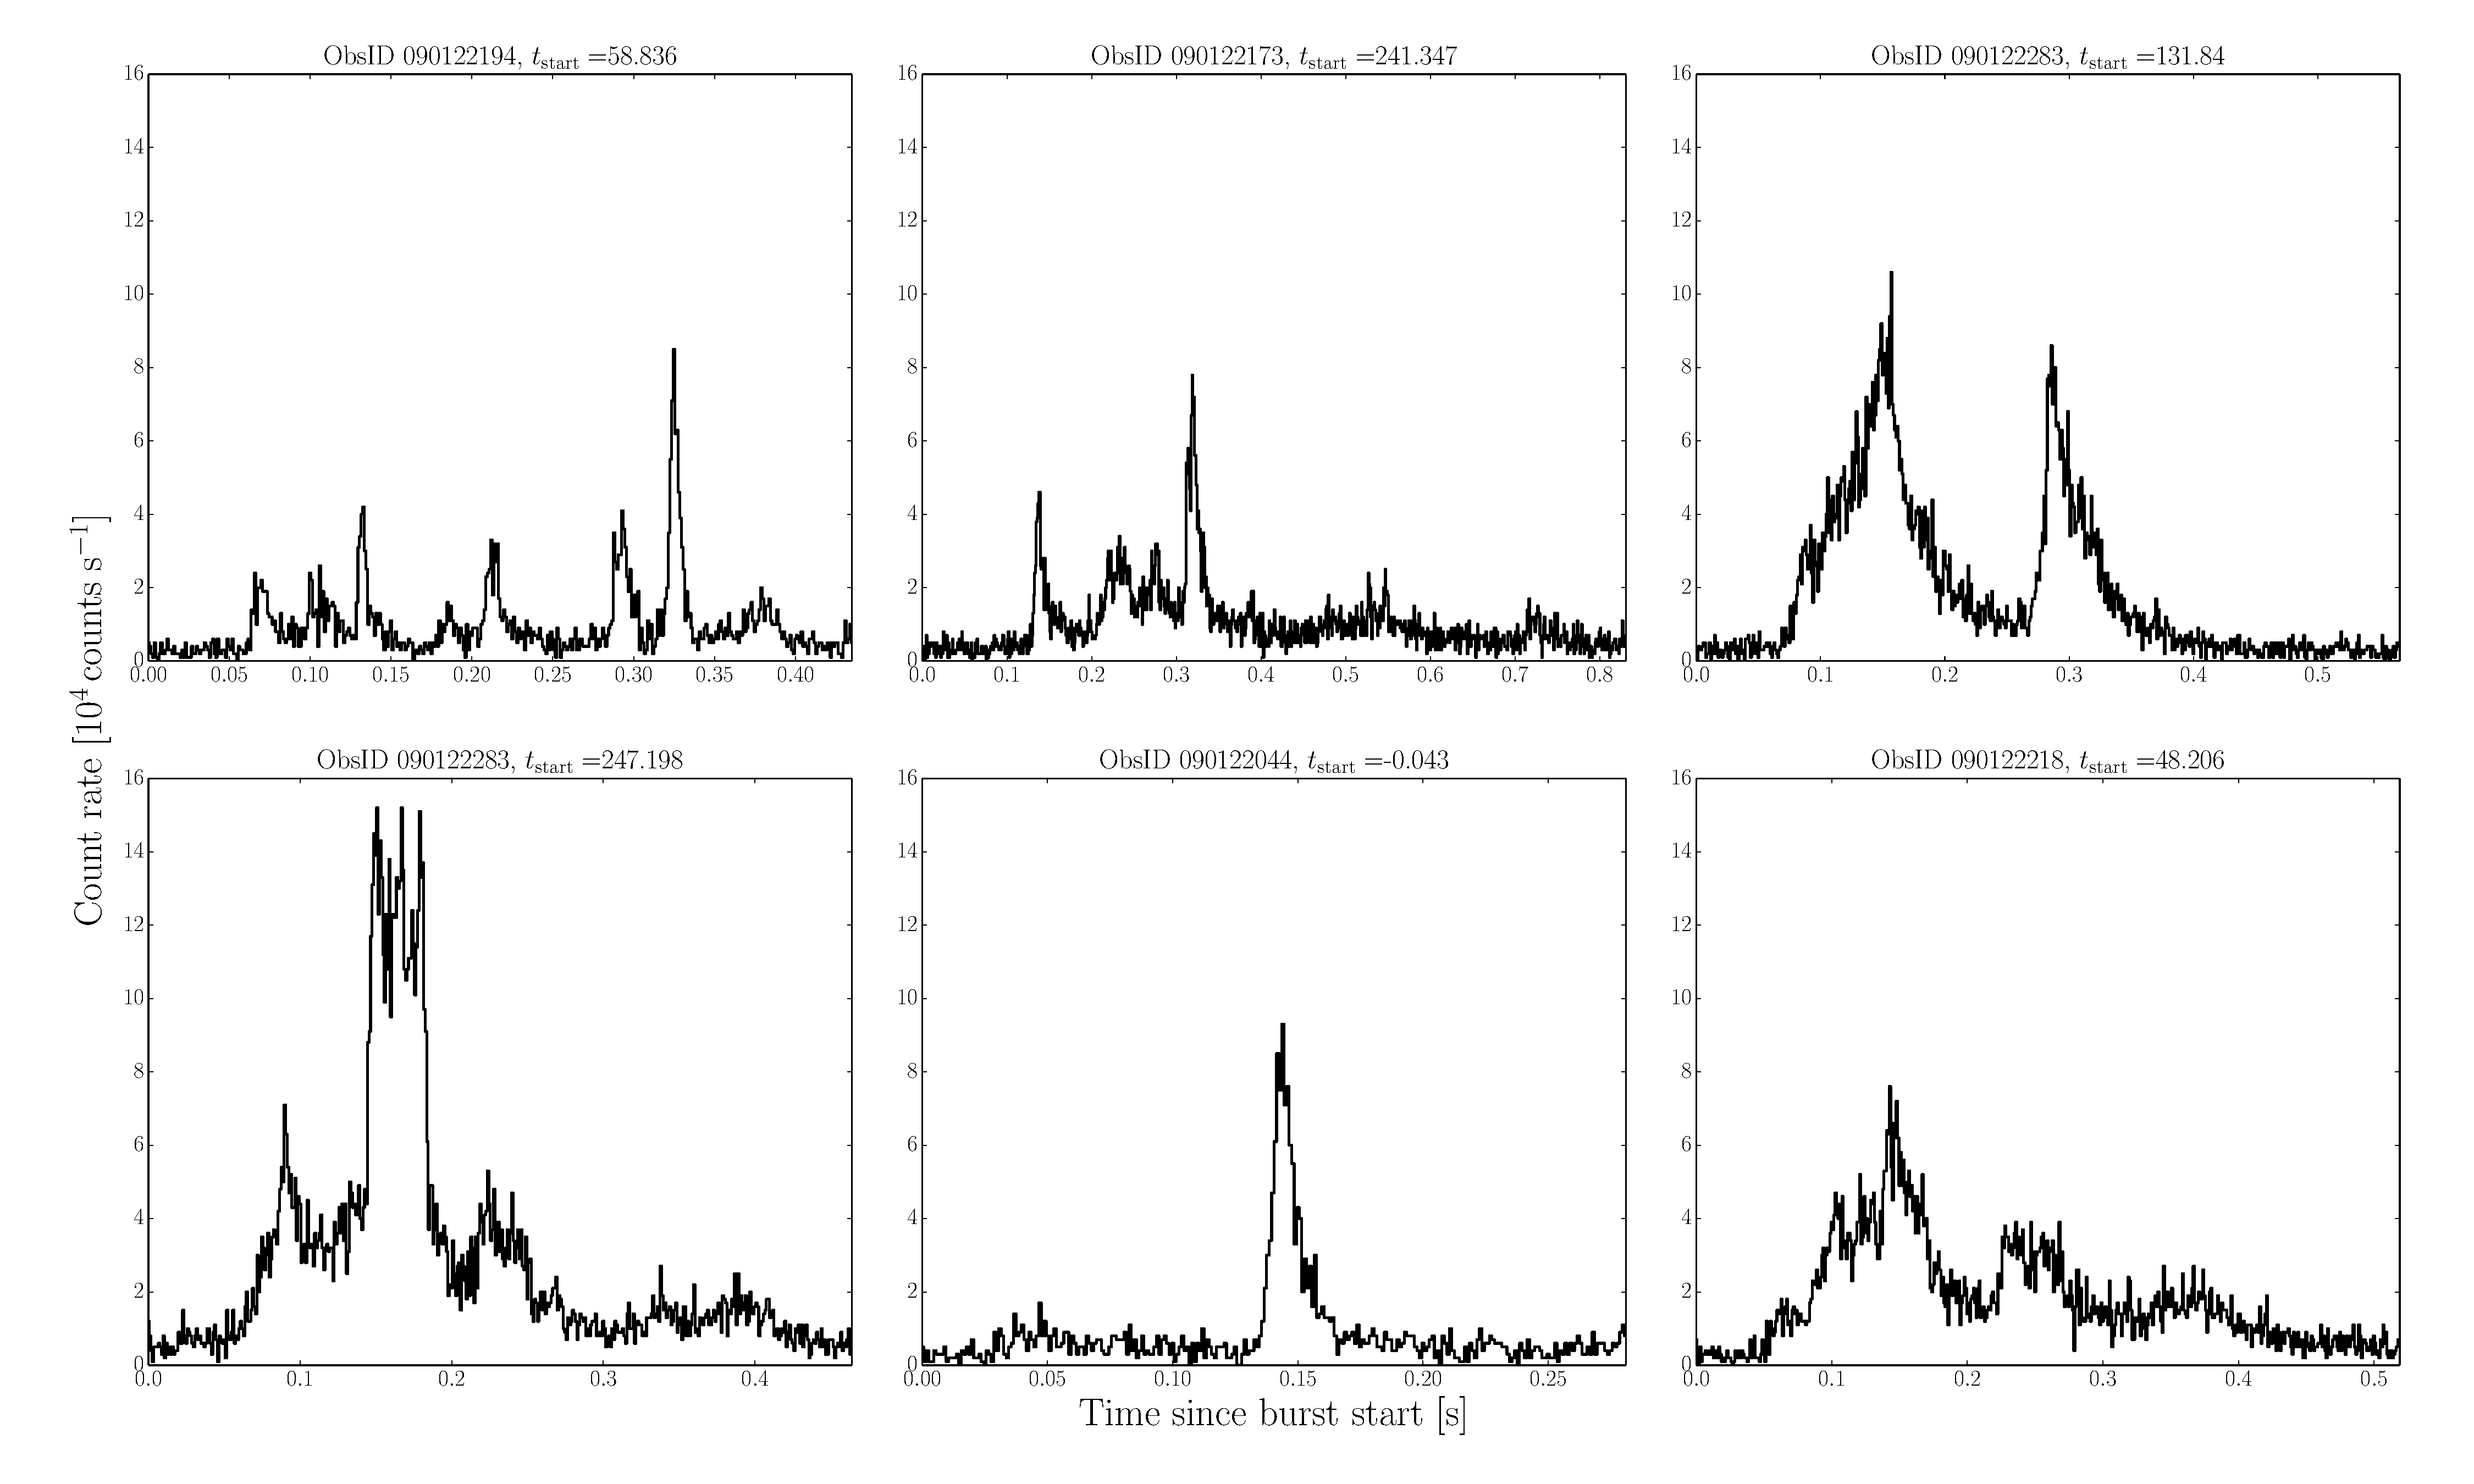
\includegraphics[width=18cm]{example_bursts.png}
\caption{}
\label{fig:example_bursts}
\end{center}
\end{figure*}

\section{Analysis Methods}

In order to successfully model the complex temporal variability in magnetar bursts, any modelling procedure must satisfy the following criteria: (1) it must be flexible enough to be applicable to a large number of bursts with distinctly different morphologies. We achieve this by decomposing magnetar burst light curves into one or more components with simple shapes, which, taken together, make up a burst. (2) the procedure must be largely automated, and be capable of sampling both the number of components as well as the model parameters for each component without human intervention. The latter is achieved by setting up a Bayesian model, where the number of components is a parameter to be sampled together with the corresponding parameters of the individual components. We use diffusive nested sampling as implemented in DNest \citep{brewer2011} to approximate the posterior distribution over all parameters. From samples of the posterior distribution,
we can then study the properties of individual burst components, as well as their properties for a given burst.

\subsection{A hierarchical Bayesian model for magnetar bursts}

For a light curve with Poisson-distributed counts $\bm{\counts} = \{\counts_i\}$ and a model $H$ we can compute the posterior probability over all model parameters in the following way:

\begin{equation}
p(N, \bm{\alpha}, }\{\bm{\theta}_i \} \given \bm{\counts}, H) = \frac{p(\bm{\counts} \given N, \bm{\alpha}, }\{\bm{\theta}_i \}, H) p(N, \bm{\alpha}, \{\bm{\theta}_i \} \given H)}{p(\bm{\counts} | H} \, .
\end{equation}

Here, $N$ is the number of model components, with the corresponding set of model components $\{\theta_i\}$. $\theta_i$ may be a scalar, for models with a single parameter, or a vector.
The scalar or vector $\bm{\alpha}$ encodes the potential hyper parameters used to describe the prior distributions of parameters in $\{\theta_i\}$. $H$ encodes the prior choices we have
made about the model that are not part of the inference problem at this stage: for example, the choice of shape for prior distributions and the model shape used to represent the light curve.

We use a Poisson likelihood to describe the data,

\begin{equation}
\likelihood(N, \bm{\alpha}, }\{\bm{\theta}_i \}) = p(\bm{\counts} \given N, \bm{\alpha}, }\{\bm{\theta}_i \}, H) = \prod\limits_{j=0}^{N}
\end{equation}


\section{Model shapes}

The model for the data in or near one burst is
\begin{eqnarray}
p(\counts_n\given\pars) &=& \Poisson(\counts_n\given\mean_n)
\\
\mean_n &=& \mean_{\bg} + \sum_{k=1}^K \mean_{nk}
\\
\mean_{nk} &\equiv& \int_{t_n-\Delta/2}^{t_n+\Delta/2} A_k\,\word(\frac{t'-t_k}{\tau})\,\dd t'
\\
\word(\xi) &=& \left\{\begin{array}{ll}\exp(\xi) & \mbox{for $\xi<0$}\\ \exp(-\xi/s) & \mbox{for $\xi\geq 0$}\end{array}\right. \, ,
\end{eqnarray}

where $\Poisson(\counts\given\mean)$ is the Poisson probability of getting count $y$ given mean rate $\mean$,
  $\pars$ is the vector or blob of all model parameters,
  $\mean_{\bg}$ is the background (DC) level in the bin,
  $t_n$ is the time of the center of the bin,
  $\Delta$ is the full width of the bin,
  $K$ is the number of words (spikes) $k$ making up the burst,
  $\phi(\xi)$ is the dimensionless word function,
  $A_k, t_k$ are the amplitudes and time offsets of the words,
  and $s, \tau$ set the shape (asymmetry or skew) and rise time of the words.
  
Various parameters can be left free completely, or can be tied together between words:
 
\begin{equation}
\theta \equiv [,\{t_k, \tau_k, A_k, s_k \}_{k=1}^K, \mean_{\bg} ]
\end{equation}

for complete freedom of word parameters between words,

\begin{equation}
\theta \equiv [,\{t_k, A_k, s_k \}_{k=1}^K,  \tau_k, \mean_{\bg} ]
\end{equation}

for tying the rise time together within a burst, and

\begin{equation}
\theta \equiv [,\{t_k, A_k\}_{k=1}^K, \tau_k, s_k , \mean_{\bg} ]\end{equation}

for a model where both the rise time and the skewness are tied together for all words within a burst.

%\begin{figure*}[h]
%\begin{center}
%\includegraphics[width=18cm]{example_words.png}
%\caption{}
%\label{fig:example_words}
%\end{center}
%\end{figure*}

  
Figure \ref{fig:example_words} shows the shape of a word
  and an example of a burst generated by our model.

The model for a large set of bursts is whatever.
[We should probably, in the above, index bursts $m$,
  and maybe even magnetar $j$.]

\emph{Notes to selves:}
At one point we figured we could \emph{fix} shape parameter $s$
  to be the same for all the words in all the bursts from one magnetar,
  but permit the duration $\tau$ to vary.
However, as we worked in our coding session we moved more in the direction
  of thinking in terms of ``rise time'' $\tau$ and decay time $s\,\tau$.
It might be better to parameterize that way.
One possible point of discovery would be that the rise times
  are fundamental to each magnetar,
  but decay times vary.
(For instance.)

The prior pdfs are
\begin{eqnarray}
p(\ln\lambda_{\bg}) &=& \Uniform(\ln\lambda_{\bg}\given a_1, a_2)
\\
p(\ln s) &=& \Uniform(\ln s\given a_3, a_4)
\\
p(\ln\tau) &=& \Uniform(\ln\tau\given a_5, a_6)
\\
p(\ln A_k) &=& \Uniform(\ln A_k\given a_7, a_8)
\\
p(t_k) &=& \Uniform(t_k\given a_9, a_{10})
\quad,
\end{eqnarray}
where $\Uniform(x\given a, b)$ is the uniform distribution for $x$ in the range $a<x<b$.

We use \project{emcee} (CITE) to perform MCMC sampling.
[We initialize the MCMC walkers how?]

Finally, there is the issue of how to set the number $K$ of words in each burst.
We take a ``cross-validation'' approach [take that, BJB],
  in which we ask what value of $K$ does the best job at making posterior predictions
  about left-out data.
[We construct this validation test how?]
Figure [what figure?] shows an example burst,
  fit with $K=1$, $2$, $3$, $4$, and $5$ words.
It also shows the result of the posterior-prediction validation
  that selects $K=4$ as the best choice for this burst.

\section{Results}

\section{Discussion}


\paragraph{acknowledgements}
We thank the organizers of MaxEnt2013.

\end{document}
